\section{Cut and count analysis}

%\subsection{optimization} 
%The following cuts are selected such that the selection signal efficiency matches that of the BDT -- could get these as well

The same varibale set as used for MVA training is employed.
The Simulating Annealing method in TMVA is used.

\begin{table} 
\begin{tabular}{l|ll} 
\hline 
variable & min & max \\ 
\hline 
% Cut values for signal efficiency: 0.300
pt	 &  5.99 & 121.05 \\ 
eta	 & -1.25 &  1.37 \\ 
fls3d	 & 16.97 & 81.03 \\ 
alpha	 &  0.00 &  0.13 \\ 
maxdoca	 &  0.00 &  0.03 \\ 
pvip	 & -0.00 &  0.07 \\ 
pvips	 &  0.21 &  1.57 \\ 
iso	 &  0.77 &  1.25 \\ 
docatrk	 &  0.00 &  0.10 \\ 
closetrk	 & -0.17 &  2.94 \\ 
chi2dof	 & -0.04 &  7.25 \\ 
\hline 
\end{tabular} 
\label{tab:cuts_barrel} 
\caption{Rectangular cut values, optimized for the {\sc barrel}, corresponding to a signal efficiency of 0.3.}
\end{table} 

\begin{table} 
\begin{tabular}{l|ll} 
\hline 
variable & min & max \\ 
\hline 
% Cut values for signal efficiency: 0.300
pt	 & 10.19 & 88.56 \\ 
eta	 & -2.01 &  2.24 \\ 
fls3d	 & 11.86 & 117.63 \\ 
alpha	 &  0.00 &  0.18 \\ 
maxdoca	 & -0.00 &  0.03 \\ 
pvip	 & -0.00 &  0.02 \\ 
pvips	 &  0.21 &  2.10 \\ 
iso	 &  0.48 &  1.08 \\ 
docatrk	 &  0.02 &  0.27 \\ 
closetrk	 & -0.16 & 15.51 \\ 
chi2dof	 & -0.04 &  3.46 \\ 
\hline 
\end{tabular} 
\label{tab:cuts_endcaps} 
\caption{Rectangular cut values, optimized for the {\sc endcaps}, corresponding to a signal efficiency of 0.3.}
\end{table} 


\begin{figure}[!h]
  \centering
  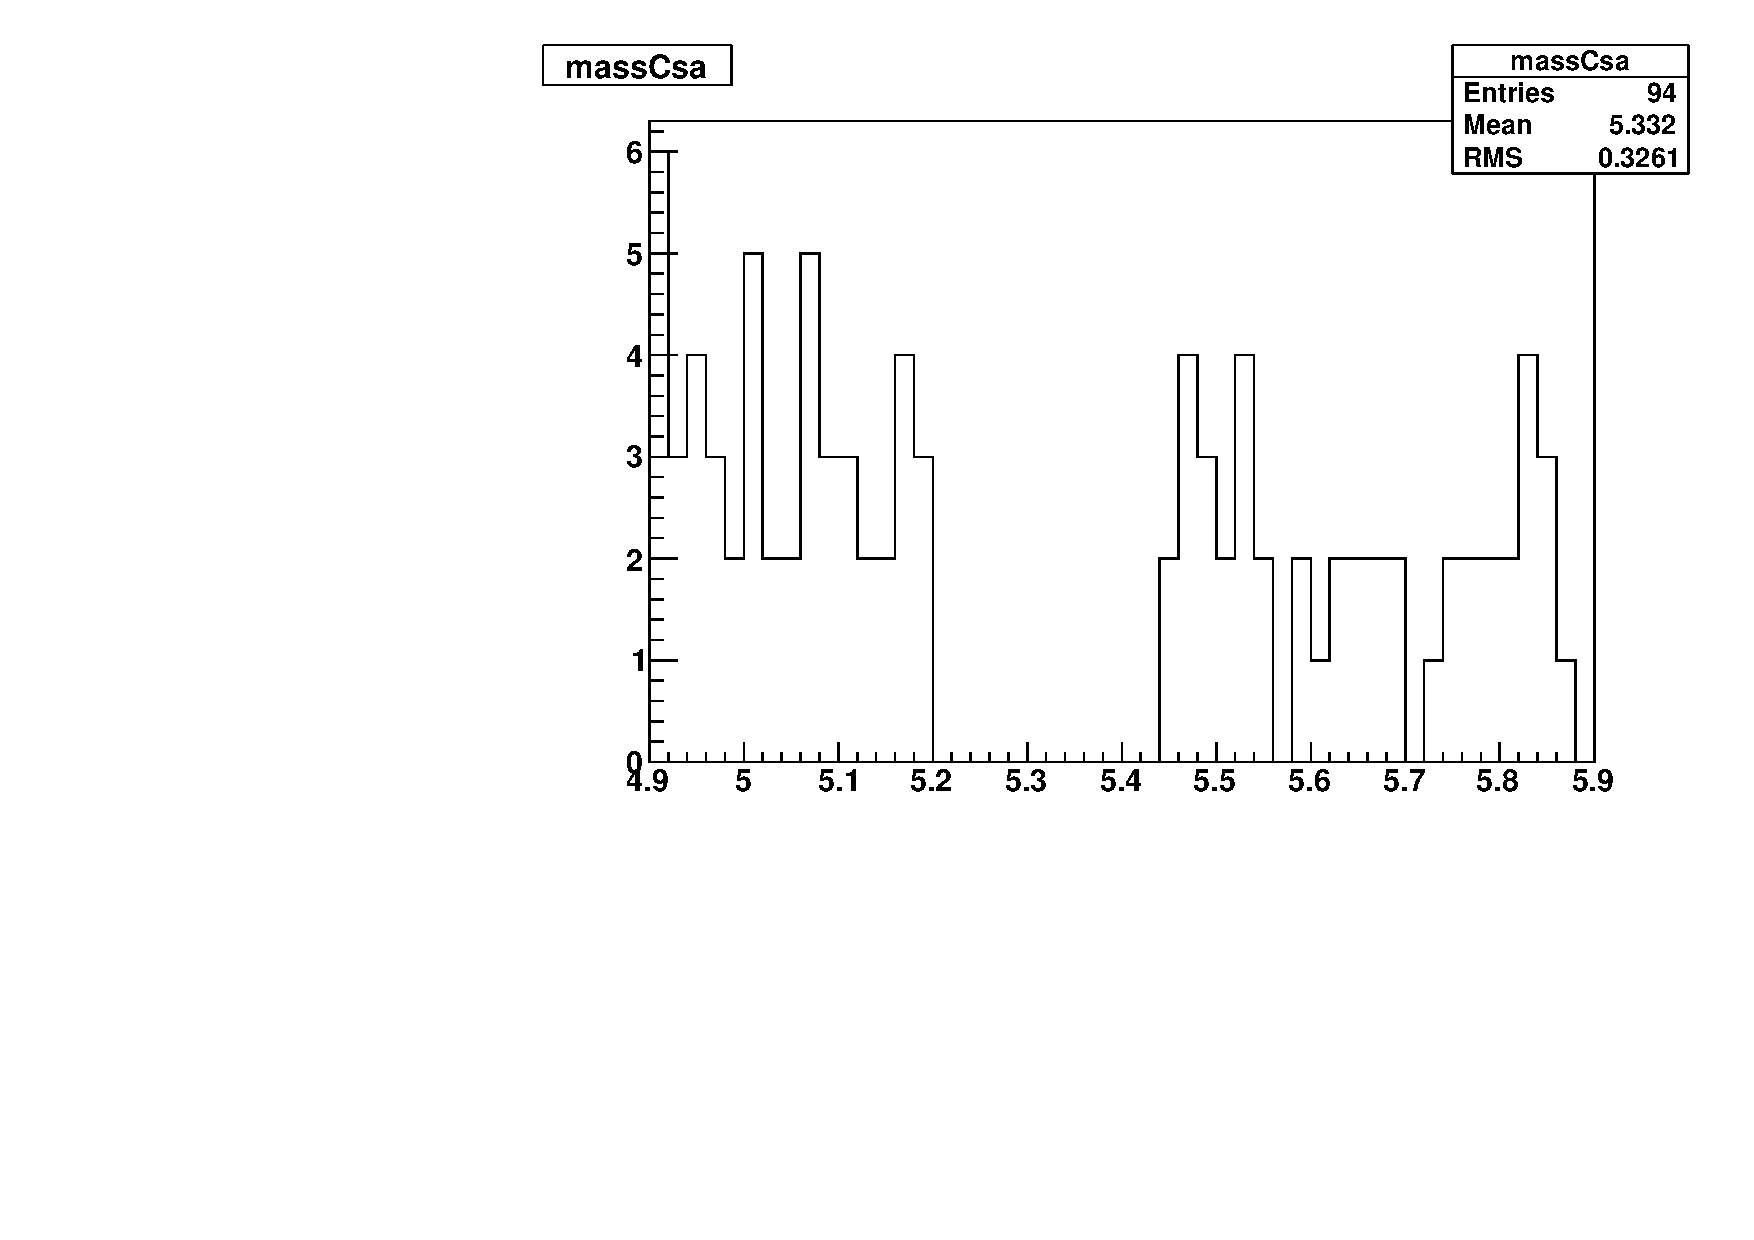
\includegraphics[width=0.45\textwidth]{Figures/cnt/SA_barrel_mass_opt}
   %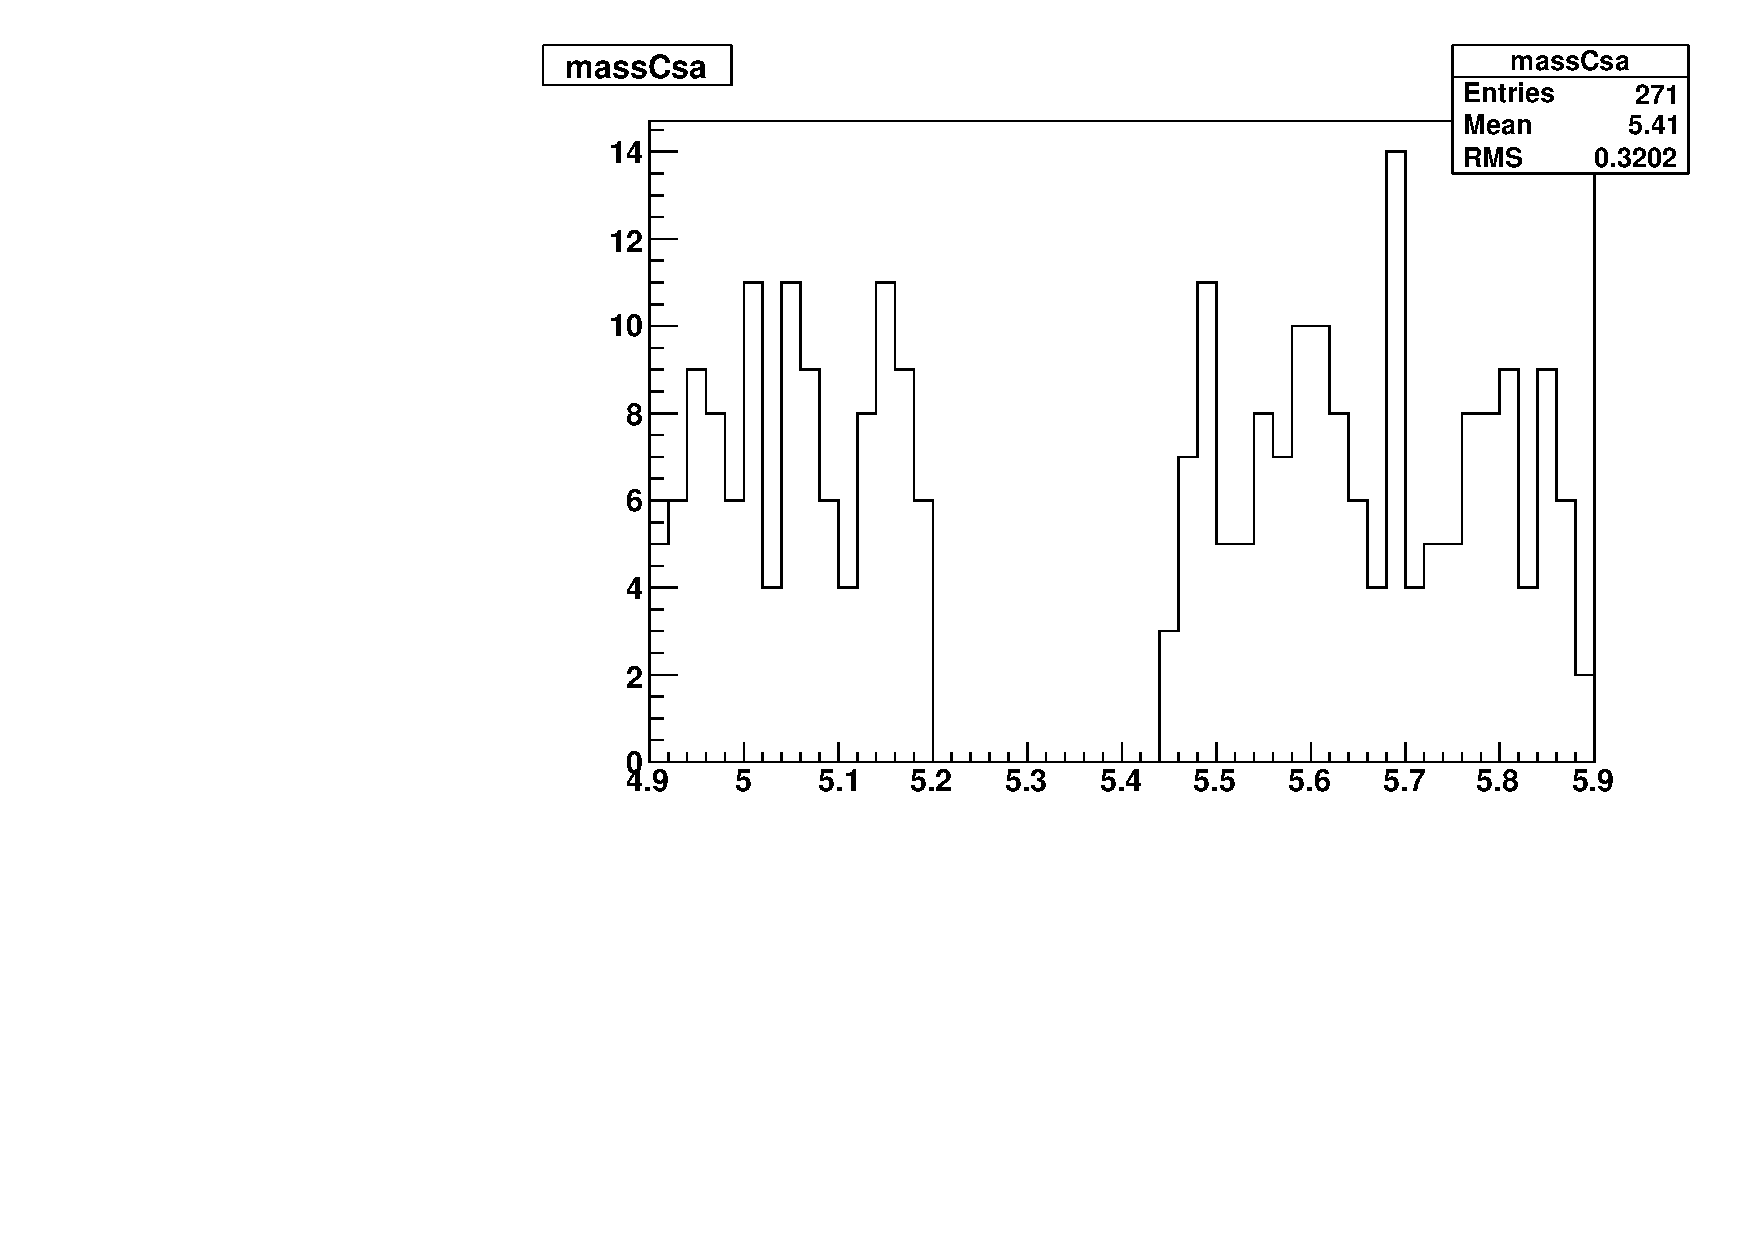
\includegraphics[width=0.45\textwidth]{Figures/cnt/SA_endcaps_mass}
\caption{Blinded cut results for barrel (left) and endcaps (right), after optimization.}
\end{figure}


%\subsection{unblind}
%
%\begin{figure}[!h]
%  \centering
%  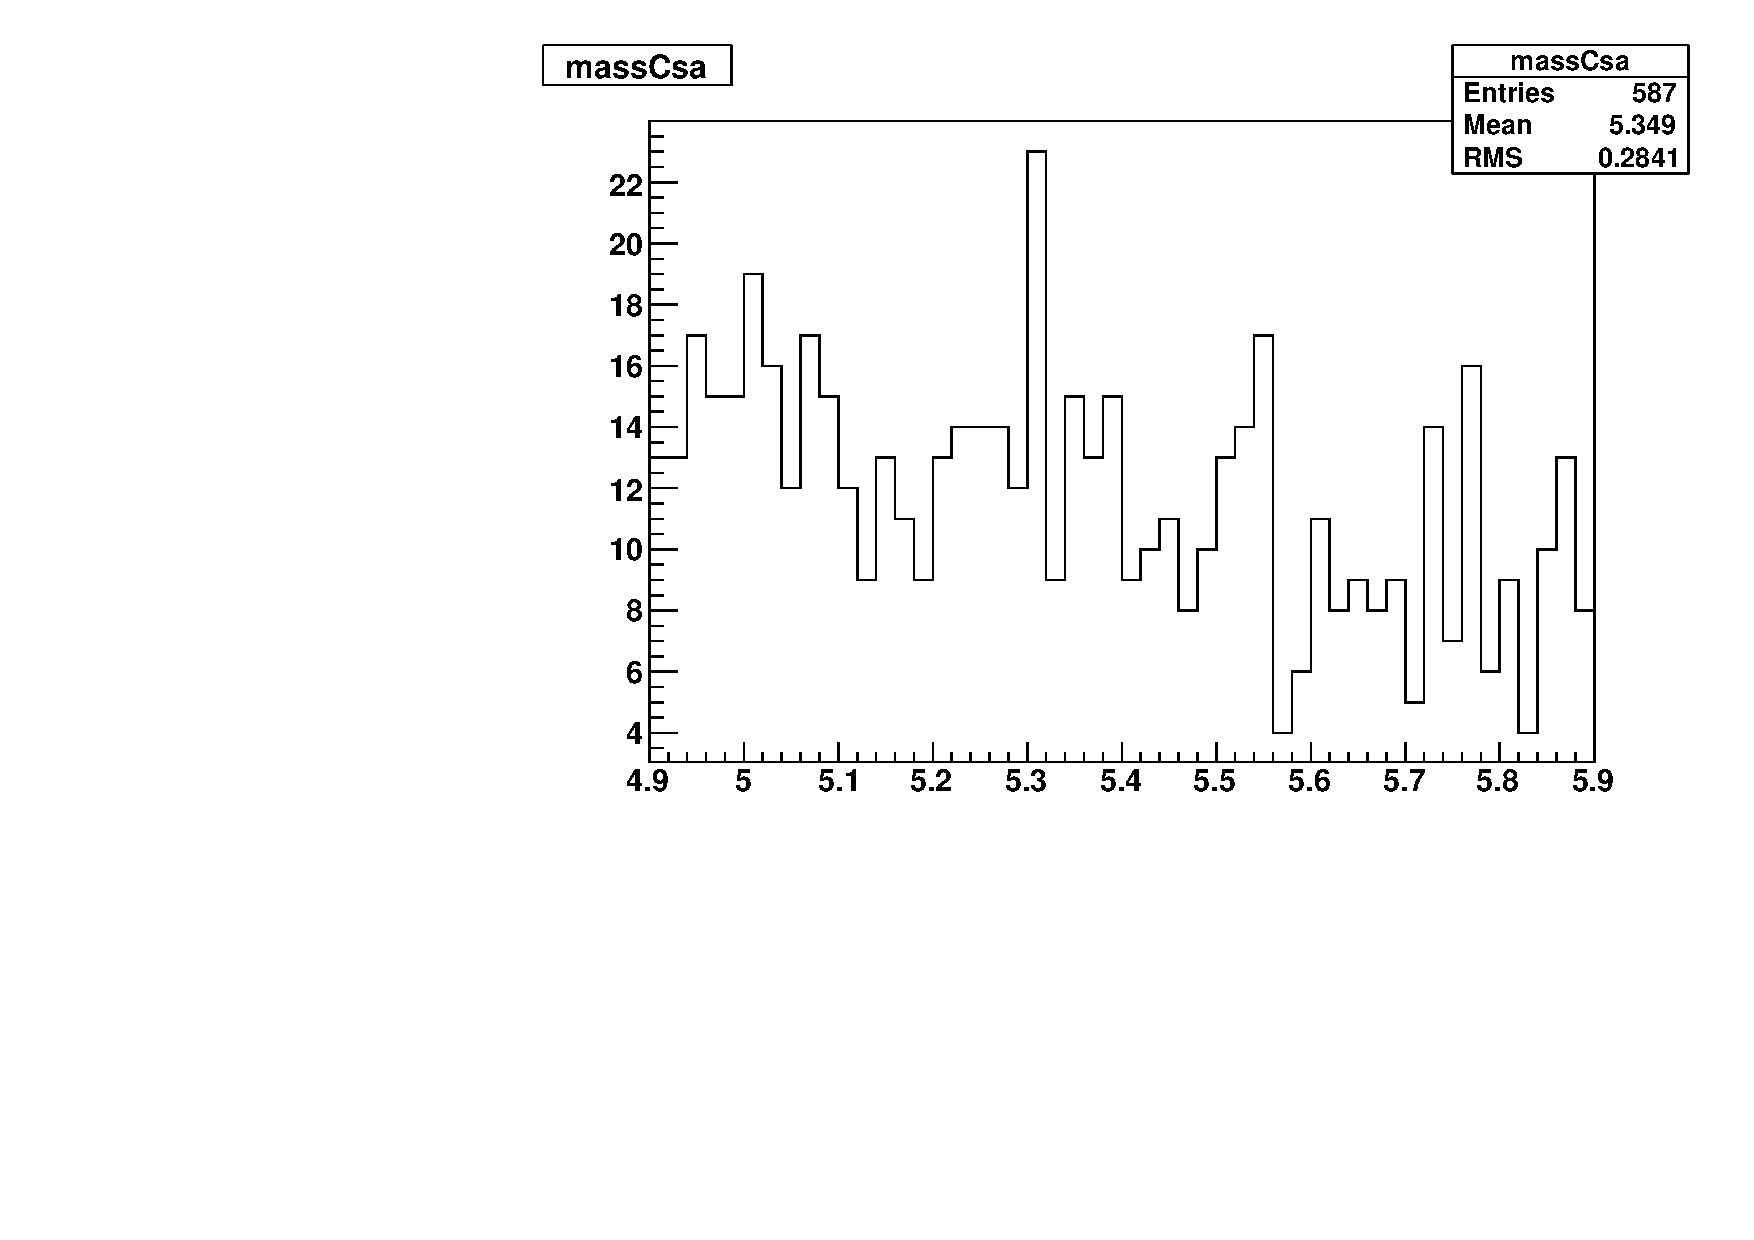
\includegraphics[width=0.45\textwidth]{Figures/cnt/SA_barrel_mass_unblind}
%  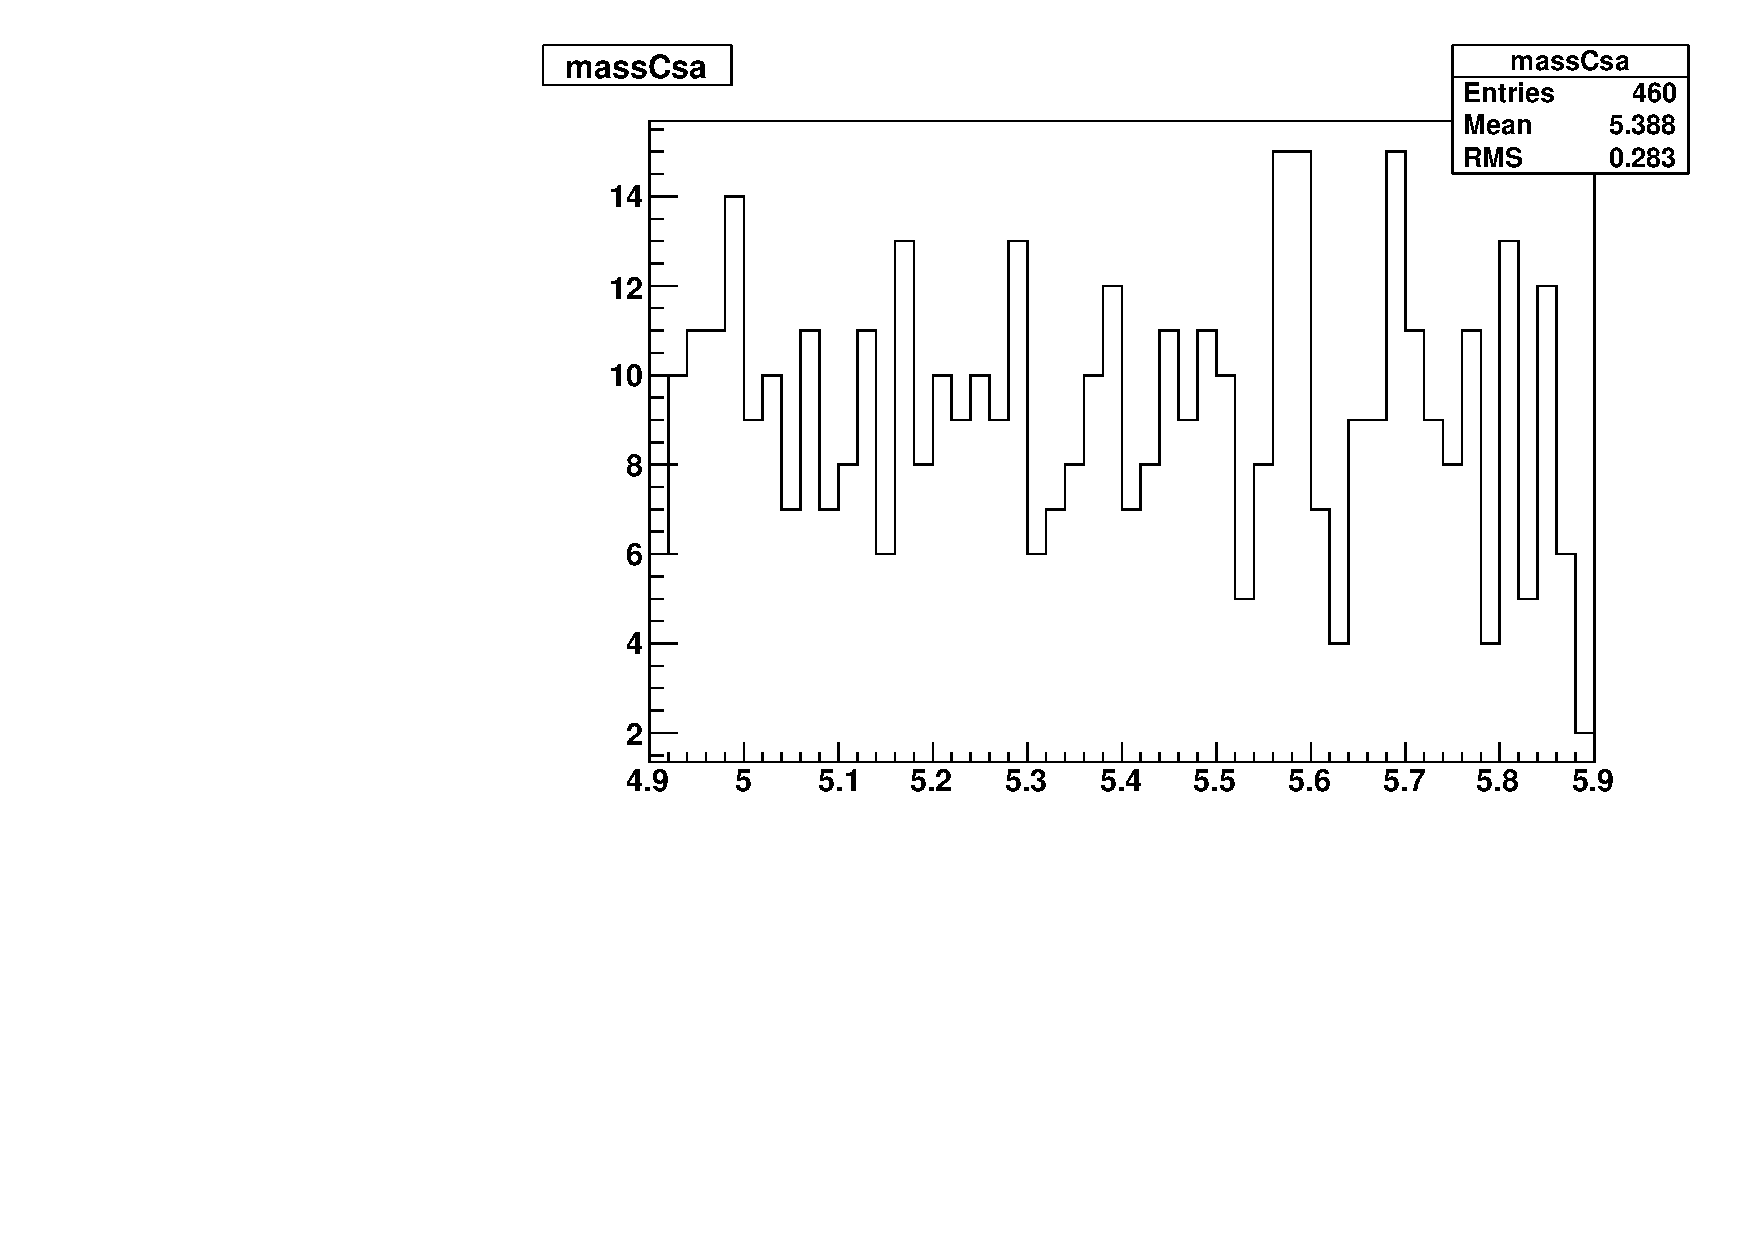
\includegraphics[width=0.45\textwidth]{Figures/cnt/SA_endcaps_mass_unblind}
%\caption{Unblinded cut results for barrel (left) and endcaps (right).}
%\end{figure}


\newpage



\begin{figure}[!h]
  \centering
  \includegraphics[width=0.45\textwidth]{Figures/barrelBDTMassPlot}
  \includegraphics[width=0.45\textwidth]{Figures/endcapsBDTMassPlot}
  \includegraphics[width=0.45\textwidth]{Figures/barrelMLPMassPlot}
  \includegraphics[width=0.45\textwidth]{Figures/endcapsMLPMassPlot}
  \includegraphics[width=0.45\textwidth]{Figures/barrelCutsSAMassPlot}
  \includegraphics[width=0.45\textwidth]{Figures/endcapsCutsSAMassPlot}
  \caption{mass plots: barrel (left) and edncaps (right); BDT (top), MLP (middle), Cuts (bottom).}
\end{figure}

\begin{figure}[!h]
  \centering
  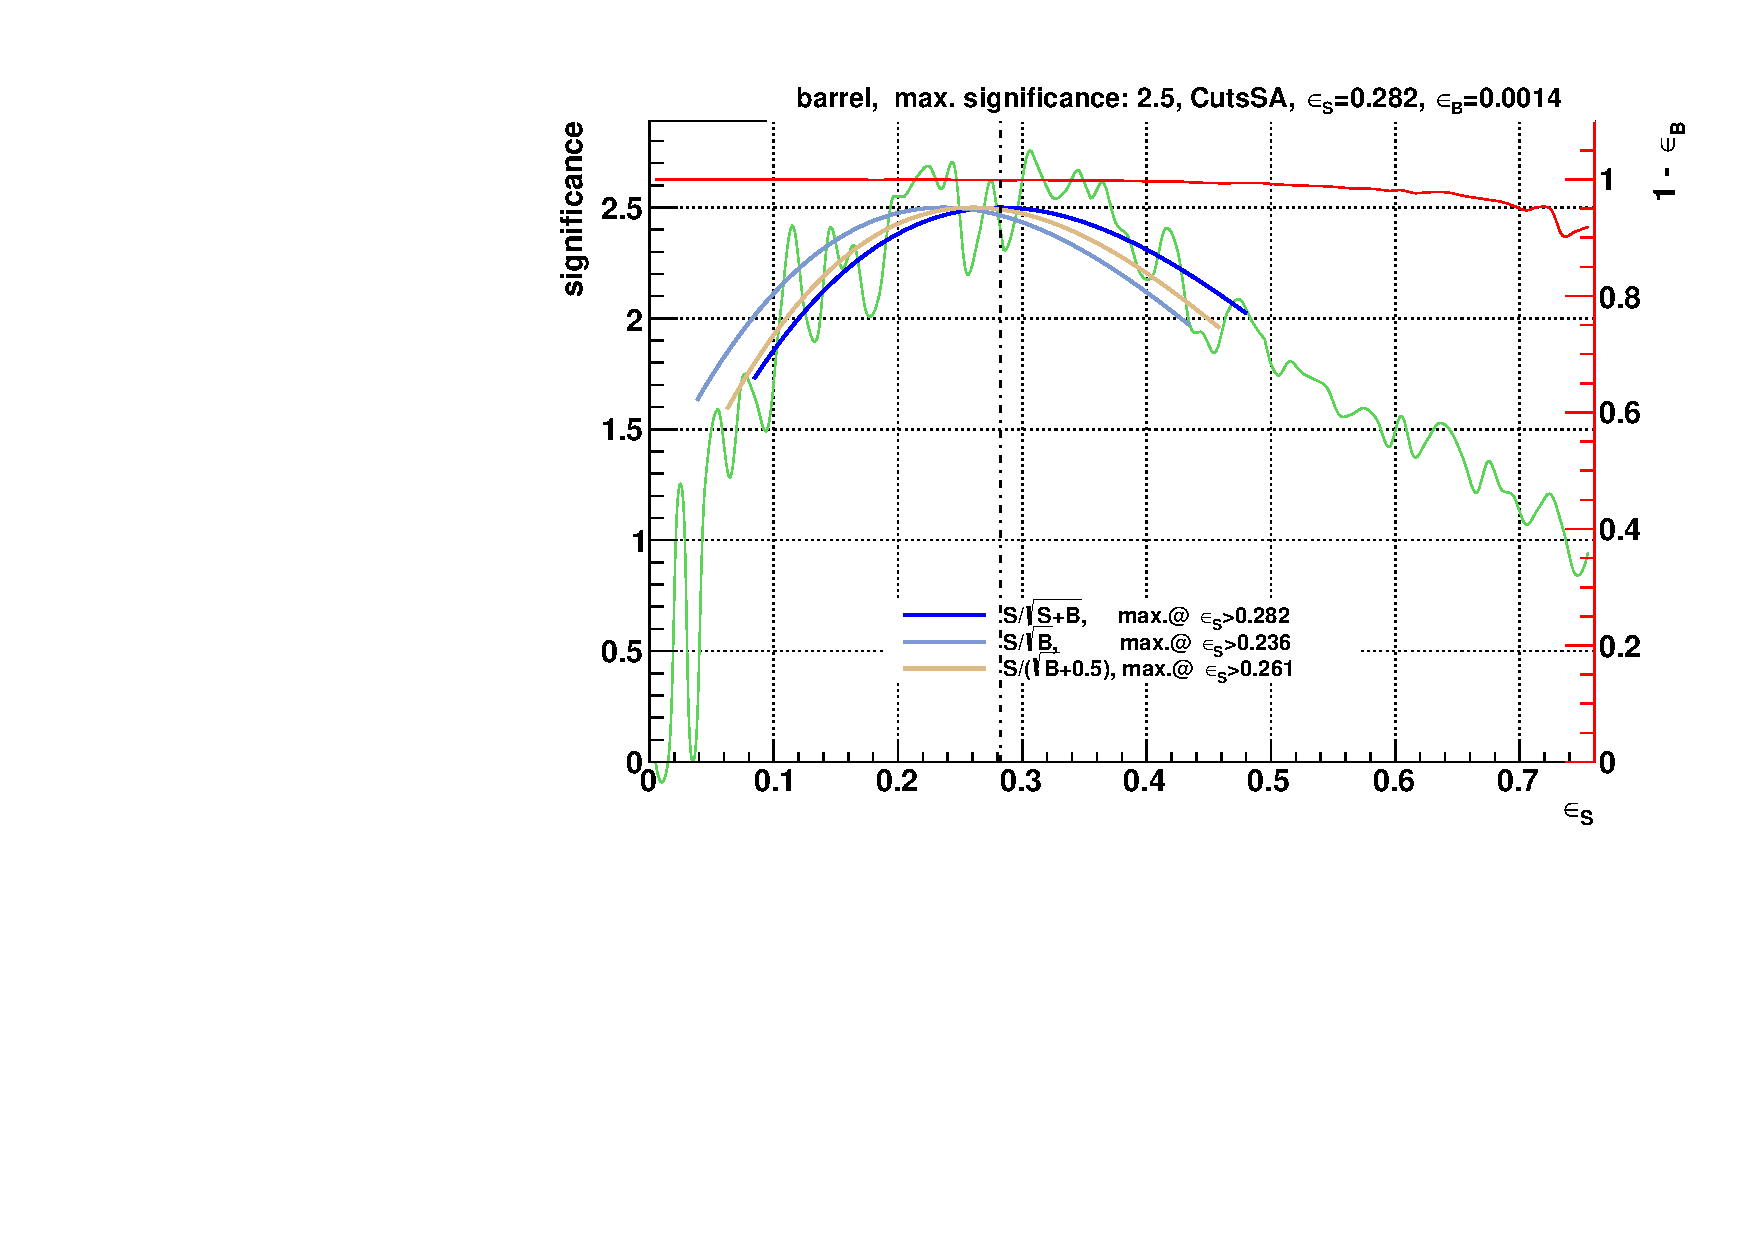
\includegraphics[width=0.45\textwidth]{Figures/cnt/CutsSA_barrel_eff}
  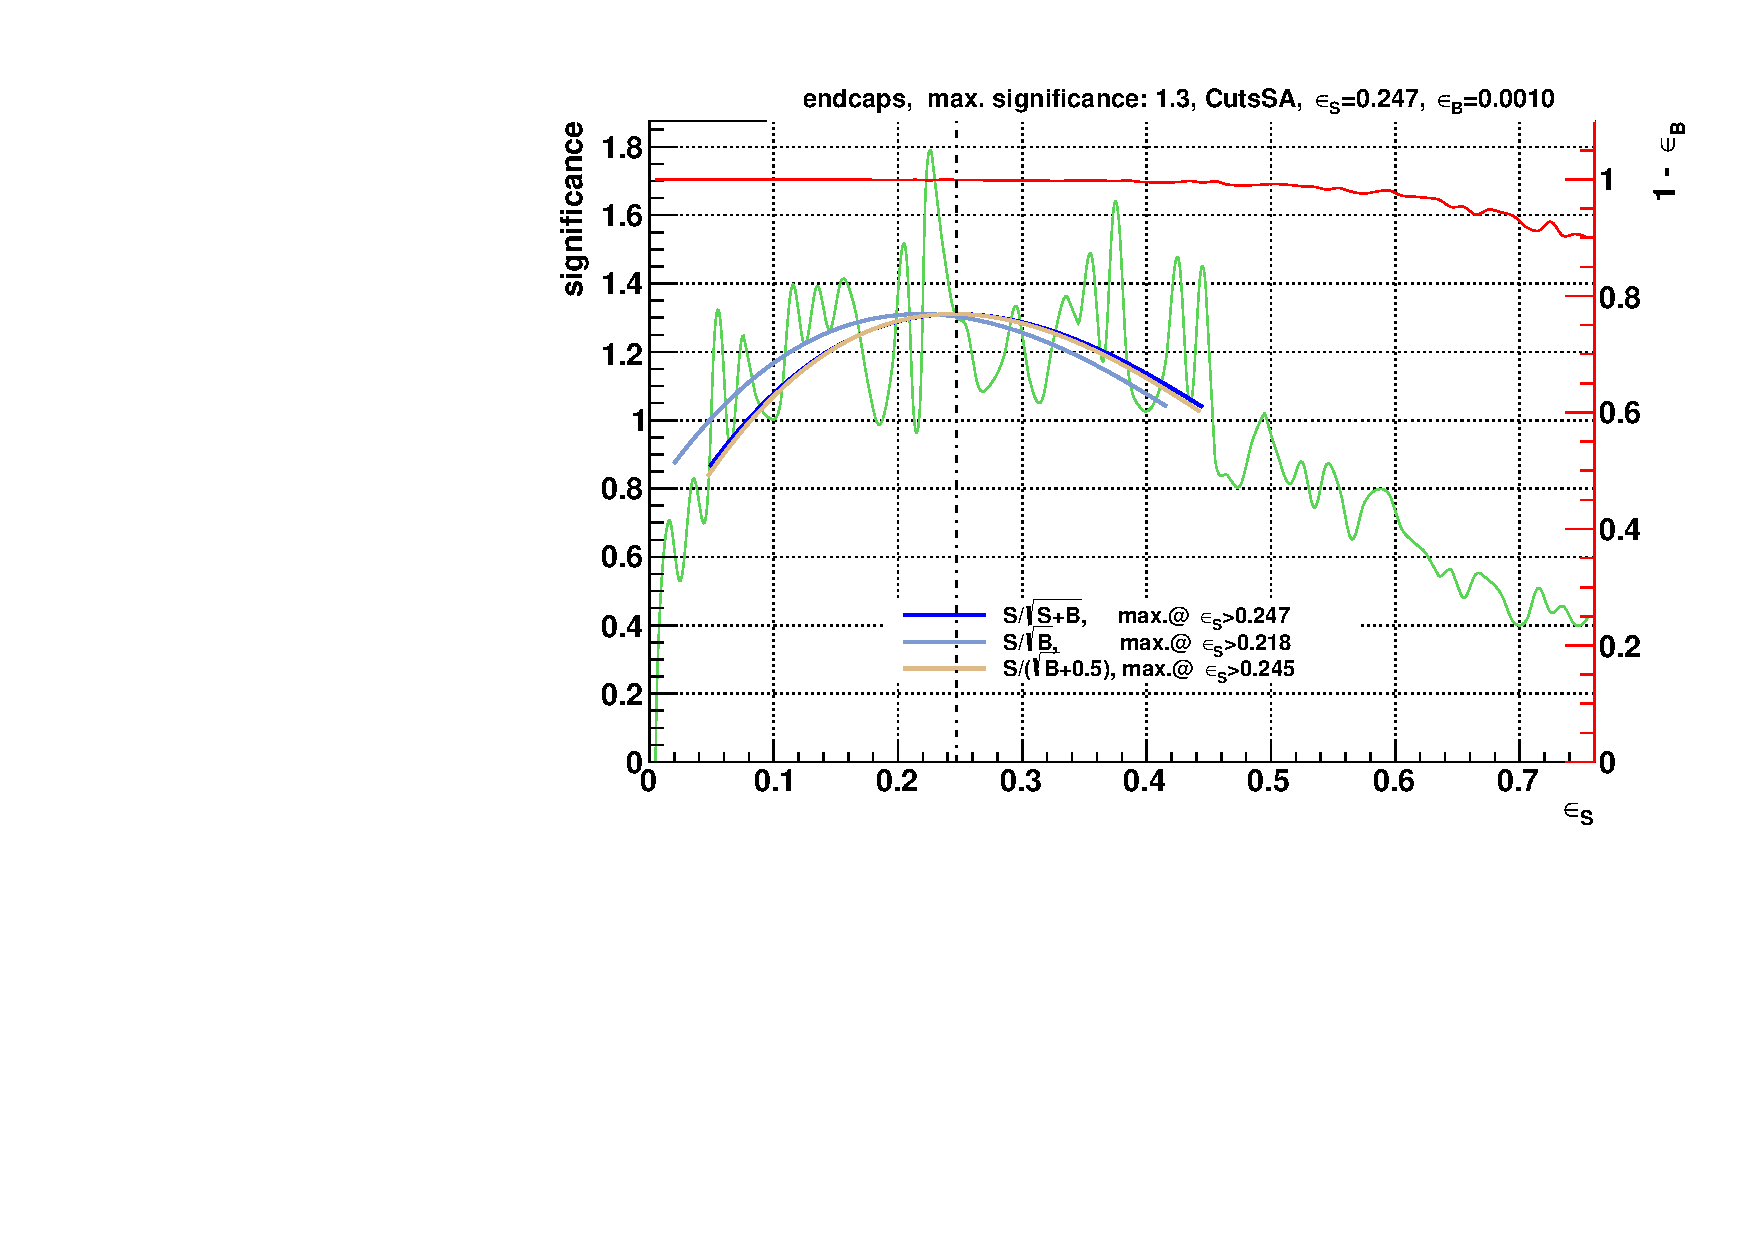
\includegraphics[width=0.45\textwidth]{Figures/cnt/CutsSA_endcaps_eff}
  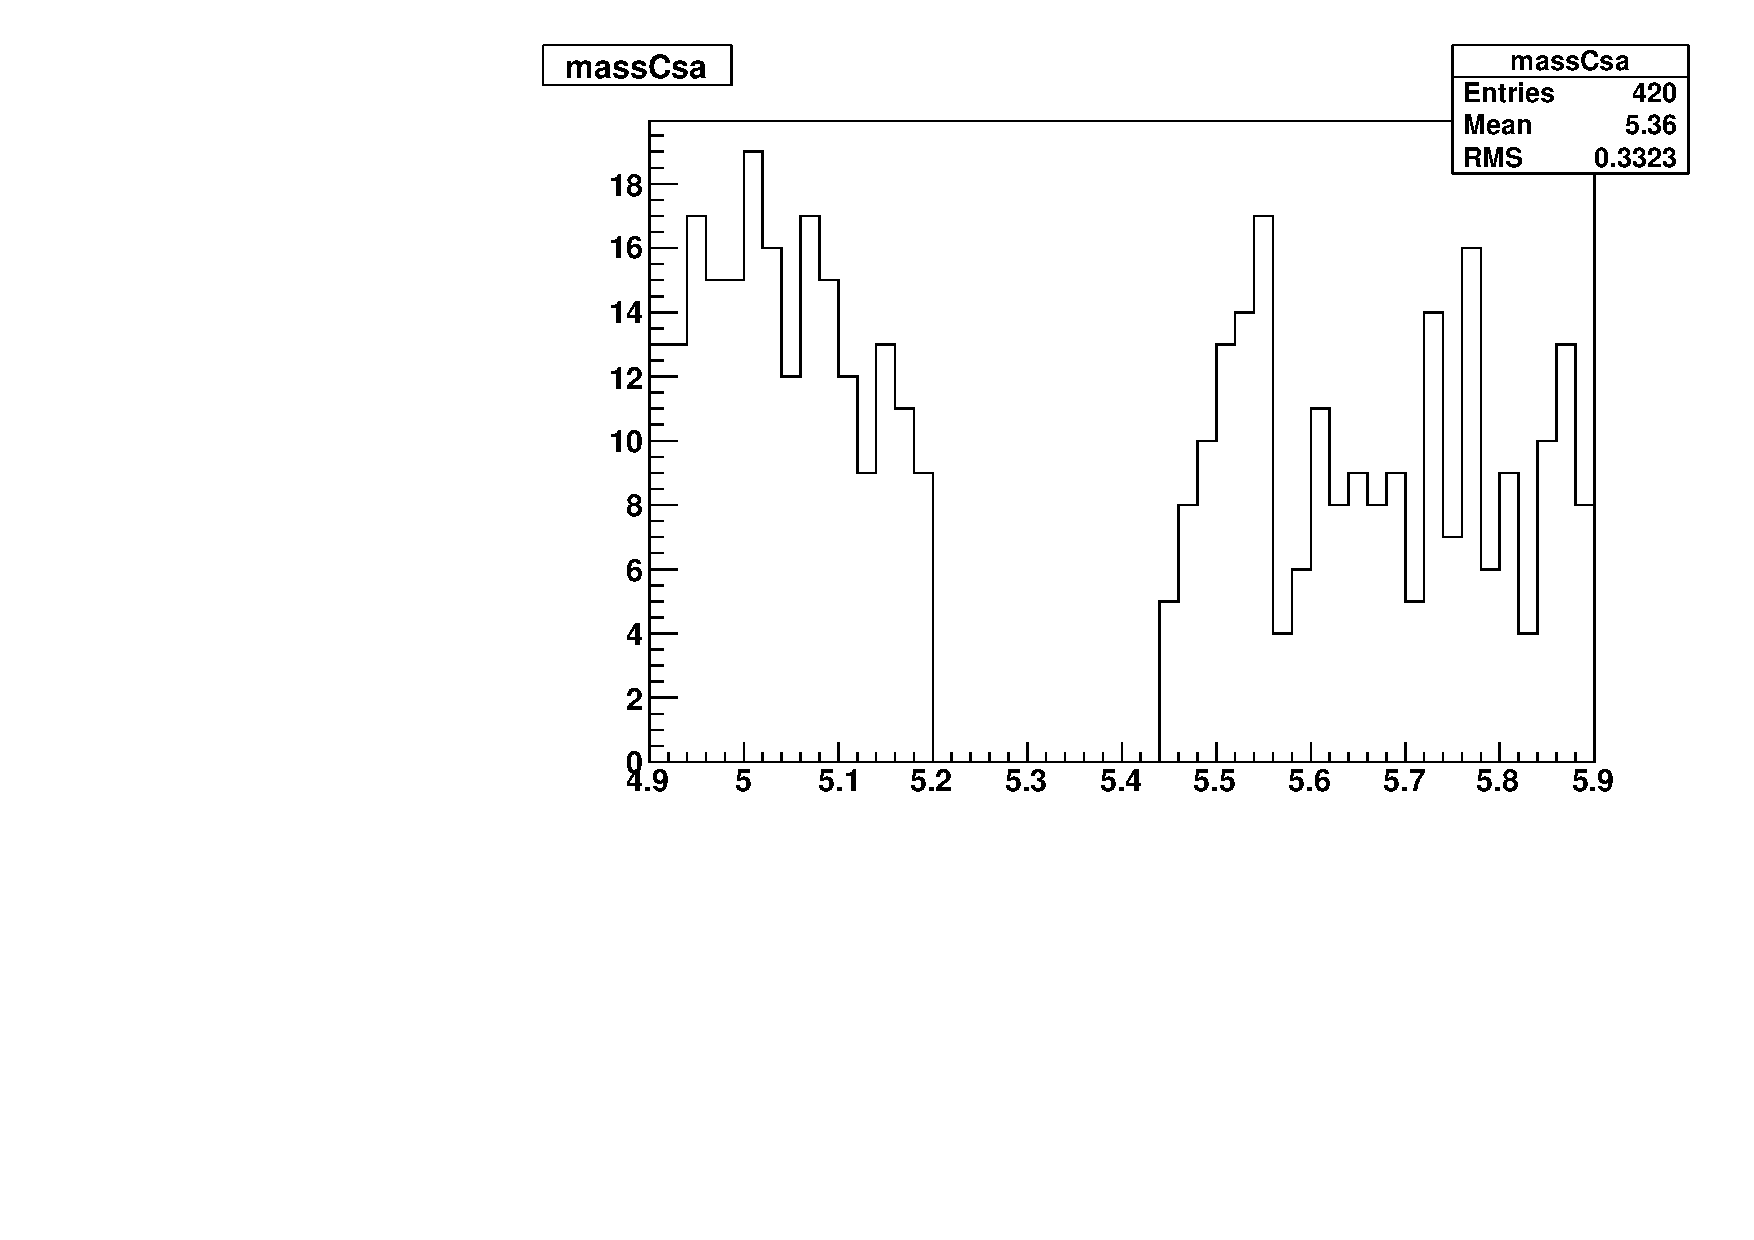
\includegraphics[width=0.45\textwidth]{Figures/cnt/SA_barrel_mass}
  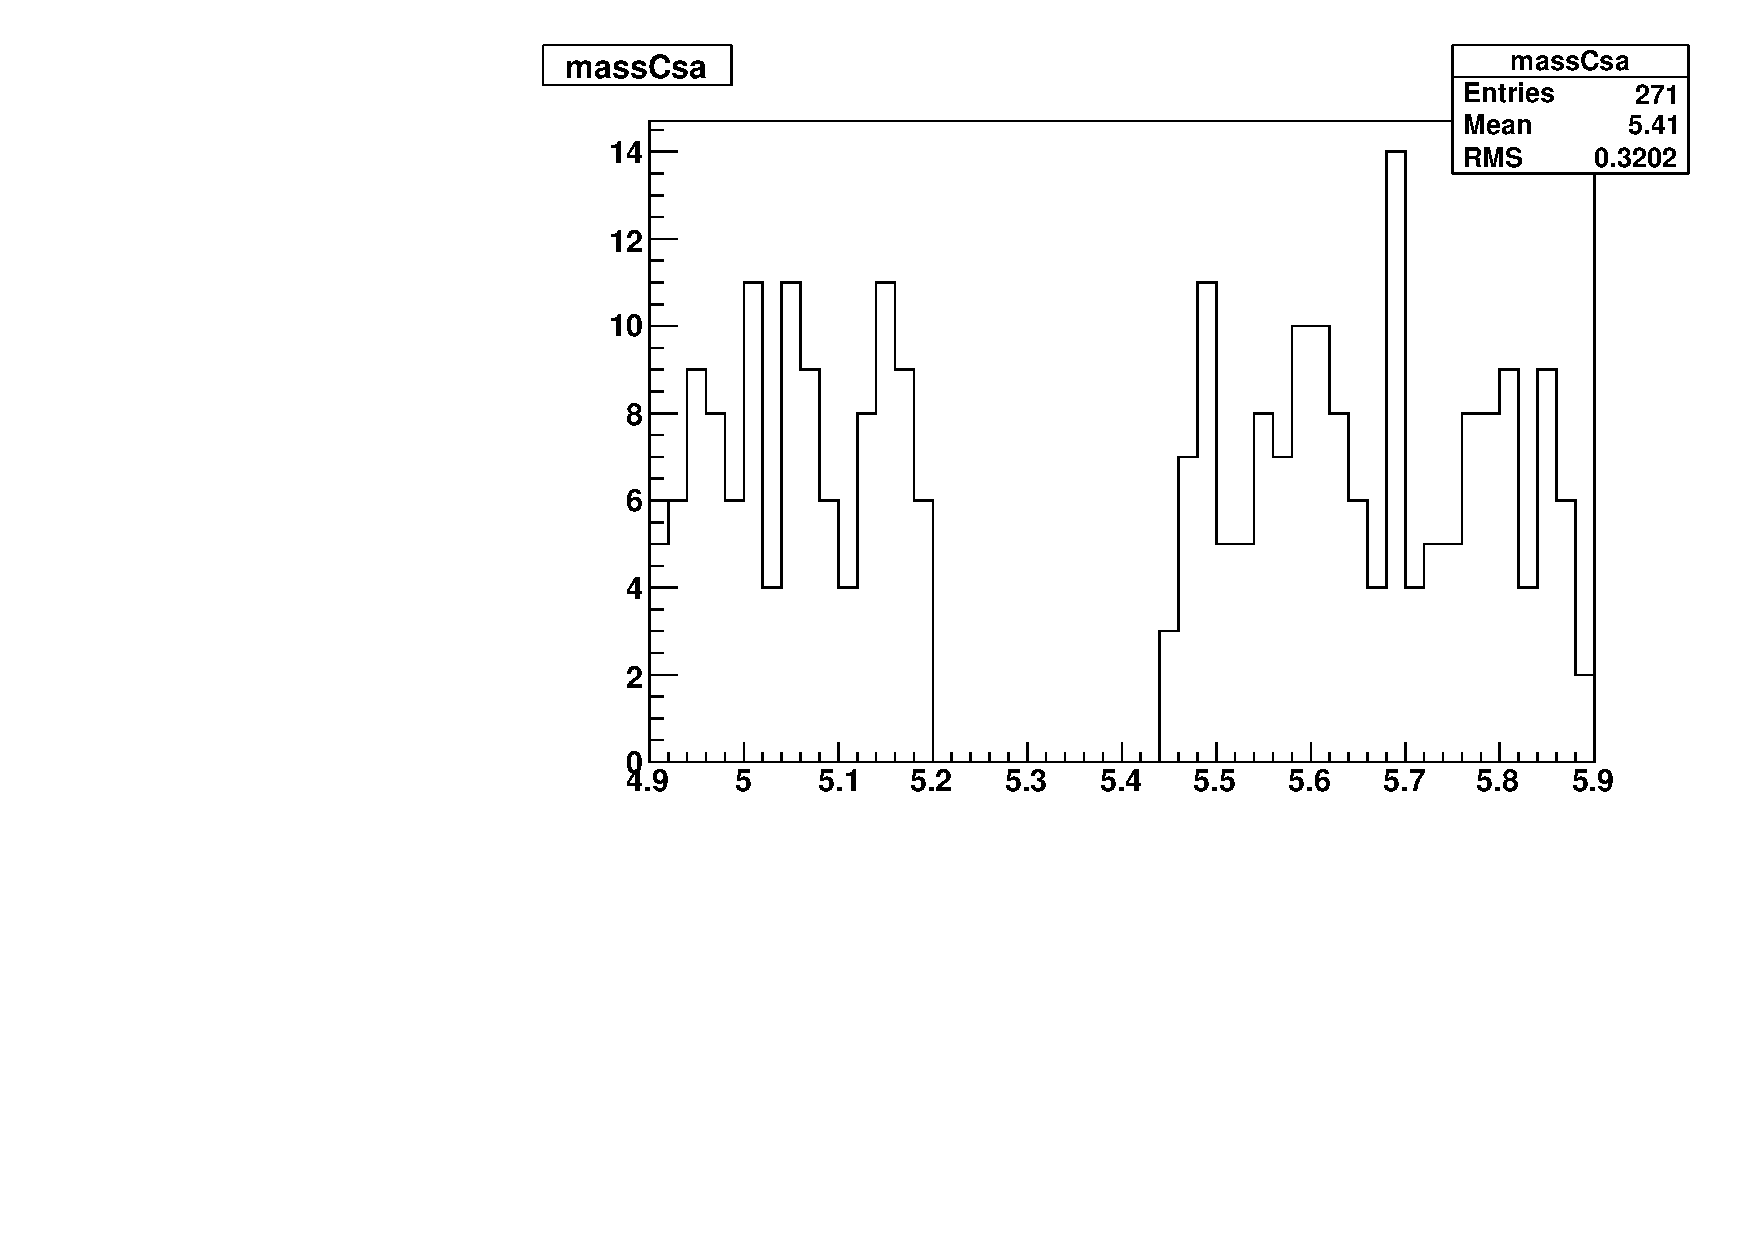
\includegraphics[width=0.45\textwidth]{Figures/cnt/SA_endcaps_mass}
  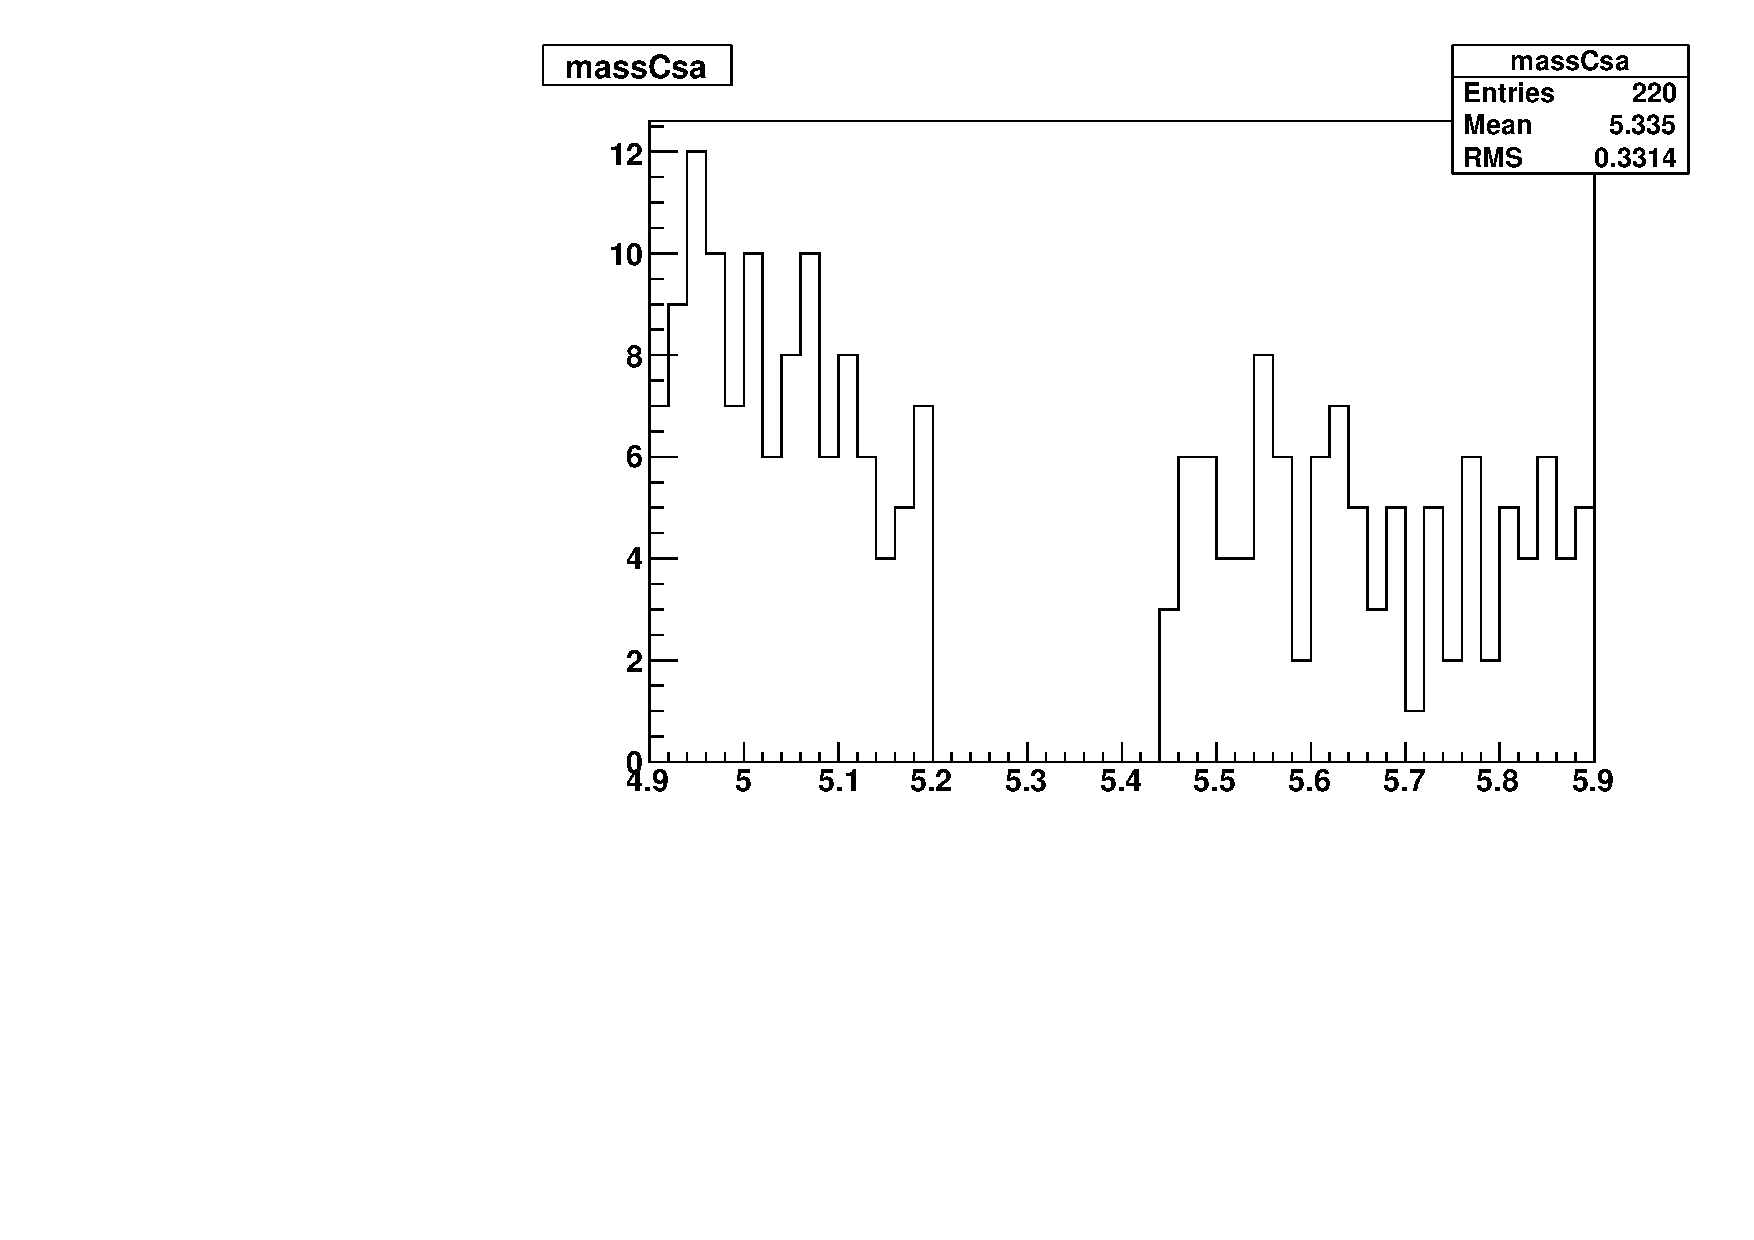
\includegraphics[width=0.45\textwidth]{Figures/cnt/mass_sa_barrel}
  \includegraphics[width=0.45\textwidth]{Figures/cnt/mass_sa_endcaps}
  %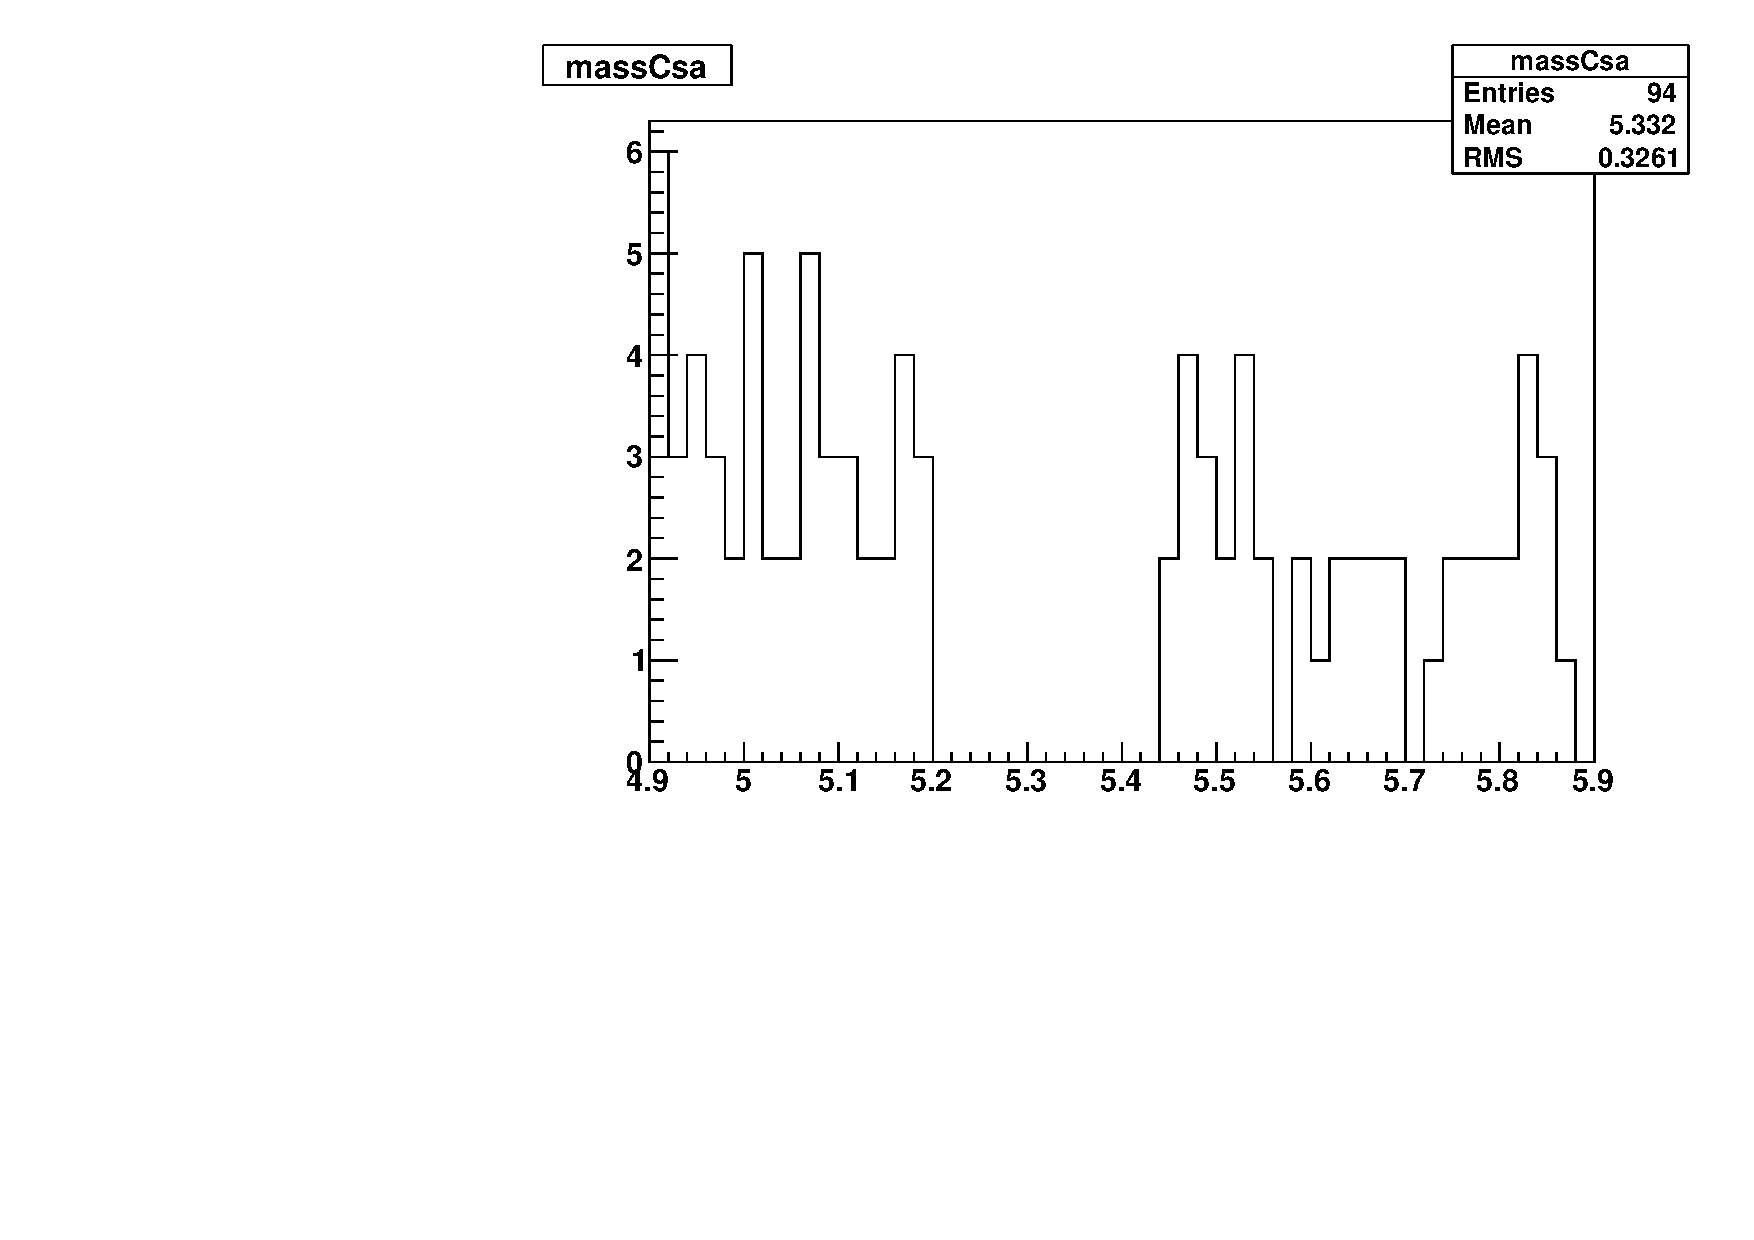
\includegraphics[width=0.45\textwidth]{Figures/cnt/SA_barrel_mass_opt}
  %\includegraphics[width=0.45\textwidth]{Figures/cnt/SA_endcaps_mass_opt}
  \caption{cut 'n count}
\end{figure}






